
\begin{frame}
  \frametitle{Parareal Dependencies}
  $
    U^{k+1}_{n+1} := G(U^{k+1}_n) + F(U^k_n) - G(U^k_n)
  $
  \vfill
  \centering
  \begin{tikzpicture}[
  text height=1.5ex,
  text depth=0.25ex,
]
  \graph[
    math nodes,
    grow right=2cm,
    diag/.style={bend left, shorten >=2pt},
  ]{
    Unk/"U_{n-1}^{k-1}" [label=above:$\vdots$]
    -> Gnk/"G(U_{n-1}^{k-1})" -> Un1k/"U_{n}^{k-1}" [label=above:$\vdots$]
    -> Gn1k/"G(U_{n}^{k-1})" -> Un2k/"U_{n+1}^{k-1}" [label=above:$\vdots$],
    "" -!- Fnk/"F(U_{n-1}^{k-1})" -!- "" -!- Fn1k/"F(U_{n}^{k-1})",
    Unk1/"U_{n-1}^{k}"
    -> Gnk1/"G(U_{n-1}^{k})" -> Un1k1/"U_{n}^{k}"
    -> Gn1k1/"G(U_{n}^{k})" -> Un2k1/"U_{n+1}^{k}",
    "" -!- Fnk1/"F(U_{n-1}^{k})" -!- "" -!- Fn1k1/"F(U_{n}^{k})",
    Unk2/"U_{n-1}^{k+1}" [label=below:$\vdots$]
    -> Gnk2/"G(U_{n-1}^{k+1})" -> Un1k2/"U_{n}^{k+1}" [label=below:$\vdots$]
    -> Gn1k2/"G(U_{n}^{k+1})" -> Un2k2/"U_{n+1}^{k+1}" [label=below:$\vdots$];

    Unk -> Fnk -> Un1k1 -> Fn1k1 -> Un2k2;
    Un1k -> Fn1k -> Un2k1;
    Unk1 -> Fnk1 -> Un1k2;
    Gnk -> [diag] Un1k1;
    Gnk1 -> [diag] Un1k2;
    Gn1k -> [diag] Un2k1;
    Gn1k1 -> [diag] Un2k2;
  };
  \node [left=5mm of Unk.center] {$\cdots$};
  \node [left=5mm of Unk1.center] {$\cdots$};
  \node [left=5mm of Unk2.center] {$\cdots$};
  \node [right=5mm of Un2k.center] {$\cdots$};
  \node [right=5mm of Un2k1.center] {$\cdots$};
  \node [right=5mm of Un2k2.center] {$\cdots$};
\end{tikzpicture}

\end{frame}

\section{Larger Rail Configurations}

\begin{frame}[b,fragile]{Duration for Larger Rail Configurations}
  \begin{table}
    \caption{\parbox[t]{0.6\linewidth}{Runtime (as reported by Slurm) of low-rank~Ros1 applied to larger Rail Configurations}}
    \begin{tabular}{%
      S[table-format=5]
      S[table-format=3]
      *{5}{S[input-decimal-markers=:,output-decimal-marker=:,table-format=2:2]}
    }
      \toprule
      && \multicolumn{5}{c}{\#Threads} \\
      \cmidrule(rl){3-7}
      {Size} & {\#Steps} & {1} & {2} & {4} & {8} & {16} \\
      \midrule
      1357 & 100 & 11:16 & 7:30 & 7:18 & 6:47 & 7:54 \\
      5177 &  10 & 10:14 & 6:14 & 4:29 & 3:57 & 4:00 \\
      20209 & 10 & 44:42 & 25:55 & 17:12 & 14:17 & 14:59 \\
      \bottomrule
    \end{tabular}
  \end{table}
  \vfill
  \begin{lstlisting}
export MY_RAIL=1357 MY_KIND=lowrank MY_N=100 MY_O=1
for c in 1 2 4 8 16; do
  sbatch --time=1:00:00 -n1 -c${c} -J lr${MY_RAIL}-c${c} seq.job
done
  \end{lstlisting}
\end{frame}

\begin{frame}[b,fragile,label=rail1357]{Rail1357}
  \begin{columns}[T]
  \column{0.6\textwidth}
  \begin{figure}
    \includegraphics<1>[width=\textwidth]{figures/slides_timeline1357_1.pdf}%
    \includegraphics<2>[width=\textwidth]{figures/slides_timeline1357_2.pdf}%
    \includegraphics<3->[width=\textwidth]{figures/slides_timeline1357_zoom.pdf}%
  \end{figure}
  \column{0.42\textwidth}
  \setcounter{beamerpauses}{3}
  \only<3->{\begin{itemize}}
    \temporal<+>{}{%
    \item
      Stage $n=384$
      \begin{itemize}
        \item
          had converged after\\ $k=7$ iterations,
        \item
          but restarts to be only 1 iteration behind stage~$n-1$,
        \item
          while also leaving the \enquote{converged} state
      \end{itemize}
    }{\item Stage 384}
    \temporal<+>{}{%
    \item
      Stages $385,\ldots, 389$ also restart\\
      but only stages $\leq 387$ stop being \enquote{converged}
    }{\item Stages $385,\ldots, 389$}
    \temporal<+>{}{%
    \item
      Stage $n=387$ reaches maximum iteration~$k=K=10$ and converges
    }{\item Stage 387}
    \temporal<+>{}{%
    \item
      Stages $388, \ldots, 406$ converge early (\ie $k < K$)
    }{\item Stages $388, \ldots, 406$}
    \temporal<+>{}{%
    \item
      Stage $n=407$ sends $F(U_{n-1}^7)$ and converges
    }{\item Stage 407}
    \temporal<+>{}{%
    \item
      Stages $408 \leq n \leq 415$ computes $U_n^8$ and converge
    }{\item Stages $408, \ldots, 415$}
    \temporal<+>{}{%
    \item
      Stage $n=416$ computes $U_n^9$ and converges
    }{\item Stage 416}
    \temporal<+>{}{%
    \item
      Stages $417, \ldots, 449$ hit $k=K$
    }{\item Stages $417, \ldots, 449$}
    \alt<+->{%
    \item
      Stage 450 had converged, restarts, and hits $k=K$
    }{}
    \alt<+->{%
    \item
      The final gap on stage~449\\ is due to synchronous\\ data transfer.
    }{}
  \only<3->{\end{itemize}}
  \end{columns}
  \vfill
  %\begin{visibleenv}<2>
  \begin{lstlisting}
  export MY_ROUNDROBIN=2 MY_RAIL=1357 MY_KIND=lowrank MY_NF=100
  sbatch -n 225 -c2 -J lr11 par.job
  \end{lstlisting}
  %\end{visibleenv}
  %MY_ROUNDROBIN=2 MY_RAIL=1357 MY_KIND=lowrank MY_NF=100 sbatch -pmedium --time=4:00:00 -n 225 -c2 -J lr11-1357 par.job
  % resulting jobid: 358690
\end{frame}

\section{Errata: Parareal Reference Solution}

\begin{frame}[fragile]
  \frametitle{Parareal Reference Solution}
  \begin{itemize}
    \item
      Thesis Figure 7.7: parareal order 4/4

      \begin{lstlisting}
MY_KIND=dense MY_NF=100 MY_OF=4 MY_OC=4 sbatch -n450 -c1 -J de44 par.job
      \end{lstlisting}
      %MY_NF=100 MY_OF=4 MY_OC=4 sbatch -pmedium --time=2:00:00 -n 450 -c1 -J d44 dense-par.job
    \item
      Better: sequential order 4

      \begin{lstlisting}
MY_KIND=dense MY_N=45000 MY_O=4 sbatch -n1 -c1 -J de4 seq.job
      \end{lstlisting}
      % MY_N=45000 MY_KIND=dense MY_O=4 sbatch --partition=long --time=2-00:00:00 -n1 -c1 -J de4-c1 seq.job
    \item
      Relative error negligible:
      \begin{minipage}{\linewidth}
      \begin{columns}[totalwidth=\linewidth]
        \column{0.5\linewidth}
        \begin{equation*}
          \frac{\norm{K_\text{par}(t) - K_\text{seq}(t)}_F}{\norm{K_\text{seq}(t)}_F}
          < 5\umach
        \end{equation*}
        \column{0.5\linewidth}
        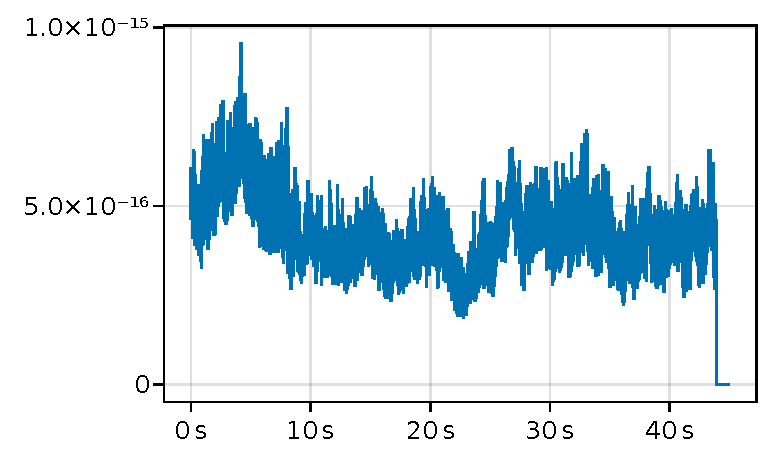
\includegraphics[width=\textwidth]{figures/slides-seq-parareal-ref.pdf}
      \end{columns}
      \end{minipage}
  \end{itemize}
\end{frame}

